% Chapter 1

\chapter{Introduction} % Main chapter title

\label{Chapter1} % For referencing the chapter elsewhere, use \ref{Chapter1} 

%----------------------------------------------------------------------------------------

% Define some commands to keep the formatting separated from the content 
\newcommand{\keyword}[1]{\textbf{#1}}
\newcommand{\tabhead}[1]{\textbf{#1}}
\newcommand{\code}[1]{\texttt{#1}}
\newcommand{\file}[1]{\texttt{\bfseries#1}}
\newcommand{\option}[1]{\texttt{\itshape#1}}
                                                 % paper



%----------------------------------------------------------------------------------------

%\section{Deep Learning for Wireless Communications}

Emotion Forecasting is the task of predicting the future emotion by comprehending the current behavioral cues. The task of traditional emotion recognition problem is to identify the current emotional state of a speaker. On the contrary, Emotion forecasting predicts the future emotional state by leveraging the audio-visual behavioral analysis from the present emotional state. Emotion forecasting is an under-explored area in the field of affective computing and to the best of our knowledge, our work is the first one that formulate and characterize the emotion forecasting problem in the deep learning domain. 

For an effective Human-Computer interaction, understanding emotional state is undeniably important. Using the audio-visual data, researchers have explored numerous aspects of emotion recognition and stepped towards more human-centered technology\cite{bla2, bla1}. On that account, with the rapid growth of smart technologies, prediction of future emotion or emotion forecasting from the current emotional state can be a promising research area. For example, in the field of predicting suicidal tendencies, Glen et. al. analyzed the short-term risk and transition from suicidal thoughts to attempts \cite{suicide2}. Therefore, in the victim to support conversation, if an intelligent agent can be developed to predict the future behavior of a suspected victim, the suicidal approach can be detected in the thought level before it reaches to the attempt level. In support to that , the work of Korrapati et. al. on social network site based suicidal prediction suggests the need for a robust and automated process of predicting sucides \cite{suicide1}. Similarly, psychiatric research on predicting a patient's behavior like anxiety or panic disorder during psychotherapy can gain several advantages from the emotion forecasting research \cite{psy1, psy2}. For example, during a psychotherapy session, the chances of giving-up of the therapy or leaving the conversation can be predicted using emotion forecasting and thus, such situation can be prevented. 

Emotion forecasting also has the potential business application. In the sector of customer care and call centers, the possibility of of success in marketing and pertaining the service quality immensely depends on customer satisfaction. Thus, forecasting of customer emotion from conversational dialog can be tremendously handy. To illustrate, in a conversation with customer while marketing for a product, if the sales agent can forecast the customer's interest or indifference, he can decide to progress the conversation or drop the conversation before the indifference turns into boredom or disgust.  Emotion forecasting can also be used effectively for automated services like chat-bots, companion robots and various intelligent agents. For instance, the user's emotion forecasting capability of Siri or Alexa can help designing more emotion specific arrangements like music or tone of conversation to comfort the user \cite{siri,alexa}.

Therefore, emotion forecasting is a potential research area in the filed of applying artificial intelligence in affective computing. In the upcoming sections, we analyze the research questions, and discuss our experimental approach and results in detail. 

The following publications were a direct result of the work presented in this thesis:
\begin{enumerate}
\item S. Shahriar and Y. Kim, "Audio-Visual Emotion Forecasting: Characterizing and Predicting Future Emotion Using Deep Learning," 2019 14th IEEE International Conference on Automatic Face \& Gesture Recognition (FG 2019), Lille, France, 2019, pp. 1-7
\item S. Shahriar, Y. Kim, B. Wang, and M. Hoai, "Early Recognition and Forecasting of Human Emotion in Audio-Visual Expressive Speech", IEEE TAFFC [in progress]
 
\end{enumerate}

\newpage
\section{Problem Formulation}
Emotion forecasting requires new problem formulation, setting-up of hypotheses, and investigation of different methods. Previous works have demonstrated the effectiveness of exploiting the temporal properties of time-varying signal for recognizing speech, emotion, and human-action \cite{speech_rec,baltru,action}. Traditional emotion recognition research showed that considering the temporal flow of emotion dynamics helps modeling the recognition system with improved accuracy \cite{kim_icassp_2013,Meta}.
This produces the first research question: Can we utilize the underlying salient information in behavioral cues to predict the future emotion? In addition to that, can sequential pattern analysis produce better insight than static pattern analysis in this case? To address this question, we present a hypothesis: \textbf{(H1)} In a dyadic conversational dialog , considering the sequential learning of information can enhance the emotion forecasting performance than in static learning. 

Previous research in the affective computing domain demonstrated that when multiple speaking utterance steps from previous steps are considered, the emotion is recognized with better performance \cite{Meta2}. This phenomena implies that emotion can occur in a longer range of time. Hence, we present our second research question: Can emotional history be useful for forecasting emotion? To address this question, we introduce the second hypothesis: \textbf{(H2)} In comparison with the history-less performance of emotion forecasting, if along with the current utterance, the previous utterance is also taken into account, emotion forecasting performance will be ameliorated.

Previous work has explored methods to predict future events from current or previous data; however, it is less explored whether and how these methods can be used in emotion forecasting. For example, forecasting of human activity \cite{Ryoo:2011:HAP:2355573.2356280}, financial event prediction \cite{TayCao}, and facial action event prediction \cite{MMED}. Hoai and Torre used partial information to detect the temporal facial actions \cite{MMED}. However, as the emotions do not have a well-defined boundary like facial actions, the implementation of the research cannot be applied directly to emotion forecasting. 
%Moreover, although emotions are expressed through many human-actions, being a slow varying signal, it holds different properties than actions.



\newpage
\section{Approach}
\label{approach}

In this thesis, as an expressive conversational dataset, we use IEMOCAP, which is segmented into variable-length utterances \cite{IEMOCAP}.
Table \ref{table:experiments} provides a detailed overview of experiments to test \textbf{H1} and \textbf{H2}. The four experimental approaches are described below: 
\begin{enumerate}
\item \textbf{UF-cur}: In UF-car approach, we forecast emotion using only the current utterance. The forecasting window is an utterance step, which means the number of speaking turns after the current speaking turn.
\item \textbf{TF-cur}: TF-cur is the time forecasting approach using only the current utterance. The forecasting window is a time range.

\item \textbf{UF-his}: In UF-his approach, emotion is forecasted by utilizing both the current and previous utterance of a speaker.

\item \textbf{TF-his}: TF-his is the same approach as UF-his but the forecasting window is time instead of utterance steps.
 
\end{enumerate}

We test our first hypothesis by experimenting with UF-cur and TF-cur approaches. We performed preliminary analysis with static models like Support Vector Machine, Random Forest, and Fully-Connected Deep Neural Network (FC-DNN), and we found FC-DNN model outperforms the other static machine learning models. Thus, we decided to use FC-DNN as a baseline static model. There are several dynamic modeling methods, including recurrent neural network (RNN) and its variants We choose to use two popular deep RNN models, namely, deep long short-term memory (D-LSTM) and deep bidirectional long short-term memory (D-BLSTM) network. 

Our second hypothesis is tested using UF-his and TF-his approaches. We explore the potential of additional history with the current data in order to forecast emotion. To further demonstrate the relevance of history information, we experiment with a randomly added utterance instead of the previous utterance. The comparison between adding random and relevant data depicts the essence of context information in forecasting emotion. 

\begin{figure*}
\centering
   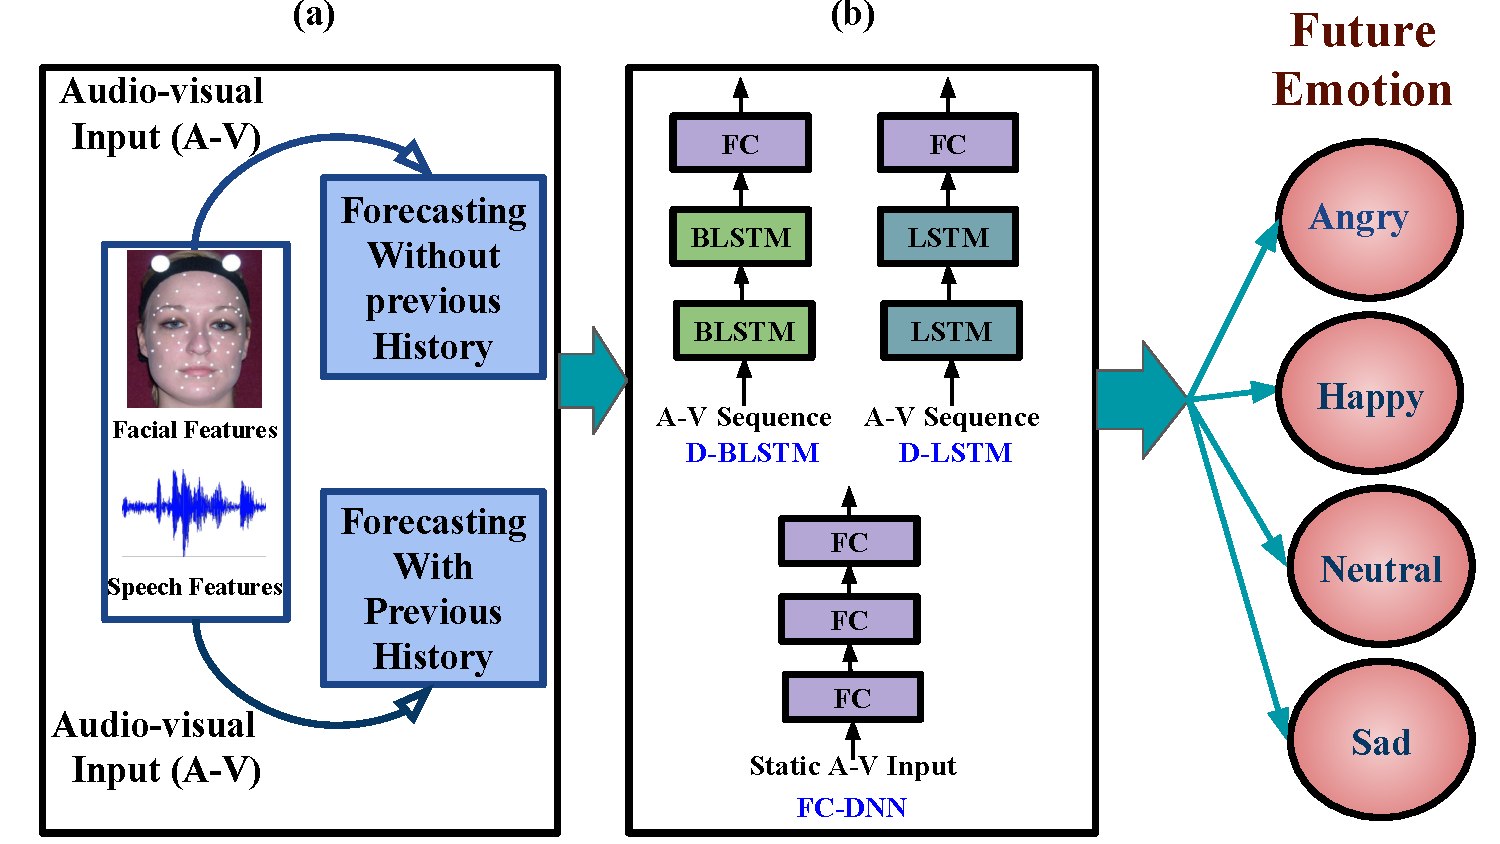
\includegraphics[width=0.9\textwidth]{overall.pdf}
\caption[Overall process of emotion forecasting]{Total process of emotion forecasting. First, in block \textbf{(a)}, we extract the audio-visual features to build up the data for emotion forecasting both in history-less and history-added setting. Next, we use static and dynamic model architecture to forecast four emotion categories. The facial figure is generated from \cite{IEMOCAP}.}
\label{fig:overview}
\end{figure*}

Fig. \ref{fig:overview} demonstrates the emotion forecasting overview. First, audio-visual features are extracted and processed in different forecasting windows. These features are fed into different deep learning models. Our analysis indicates that the temporal analysis of behavioral cues with the history context can provide the better insights for future emotion prediction. 


\begin{table}[h]
\centering
\caption{Experimental approaches for evaluation of \textbf{H1} and \textbf{H2}. The UF-cur and TF-cur approaches are used to test \textbf{H1}, and the remaining approaches are used to test \textbf{H2}.}
\begin{tabular}{|l||c|c|c||}\hline
\diagbox[width=15em]{\textbf{Forecasting} \\ \textbf{Window}}{\makecell{{}\\\textbf{History}}} &
  \makecell{History-less \\(cur)} & \makecell{History-added \\(his)} \\ \hline
\hline
\makecell{Utterance Forecasting \\ (UF)} & UF-cur & UF-his\\
\hline
\makecell{Time Forecasting\\ (TF)} & TF-cur & TF-his  \\
\hline
\end{tabular}
\label{table:experiments}
\end{table}


\begin{table}[h]
\centering
\caption{Proposed and baseline experimental models for testing \textbf{H1} and \textbf{H2}.}
\begin{tabular}{ l l}
\hline
\textbf{Static Model } & \textbf{Temporal Model} \\
\hline
\hline
\multirow{2}{*}{FC-DNN} & D-LSTM \\
          & D-BLSTM \\
\hline
\end{tabular}
\label{table:models}
\end{table}

\newpage
\section{Related Works}
\label{related_works}
Forecasting the future event has been studied in the fields related to emotions. In human action recognition, Davis and  Tyagi \cite{Davis:2006:MHA:1709251.1709302} presented a comparative probabilistic inference framework for a reliable human activity classification. Their work was to address the issue of rapid detection of human actions with low error rates. They focused on low-latency recognition with shortest video exposure. A similar work was conducted by Ryoo \cite{Ryoo:2011:HAP:2355573.2356280}, where he developed a bag-of-words model by leveraging the sequential nature of human activities. He tried to infer ongoing activities which leads to detect the even before it finished with time-dependent feature distribution. Early event detection is studied by Hoai and Torre \cite{MMED}, where they used structured-Output Support Vector Machine (SOSVM) to introduce Max-Margin Early Event Detectors (MMED). Using MMED, they tried to detect and localize an event before its completion. In comparison with other even detectors, such as, Support Vector Machine SVM) or Hidden Markov Model (HMM), their method was faster and more reliable. In the field of emotion recognition, Kim and Provost \cite{Kim2016EmotionSD} investigated time and duration pattern of emotional utterances. They analyzed the performance of emotion recognition by using only a portion of the emotional utterance. Their work drives us to hypothesize that emotional effect can be foreseen from longer distances than only a specific utterance. W\"{o}llmer et al. \cite{Meta2} explored the effect of including the past and future utterances along with the current one to recognize the emotion. However, their inclusion of future utterance to boost the D-BLSTM performance contradicts our purpose of timely-manner recognition of emotion. Therefore, we focus on forecasting, where we use the present and past temporal data to predict the future emotional state, and do not use the current utterance to make the system robust and efficient. 

The fields not directly related to emotion also performed the task of forecasting by leveraging the machine learning techniques. Kiratzis et. al. developed an ANN based short-term load forecasting model \cite{loadForecast}. They predicted the daily load curve in an autonomous power system. The forecasting of future event was also investigated in financial data research. Tay and Cao presented a comparative analysis on applying SVM and NN in financial time series. 

Although forecasting actions or events from previous data were analyzed in many fields, predicting future emotion has not been explored much, with the exception of \cite{norozi}. The sequence of emotional state was predicted in a closer work by Noroozi et al. In their work, they manually concatenated four emotional speech and annotated as boredom, fear, joy and sadness and formulated a time series. A nonlinear autoregressive model was used to predict the next emotional group from the learned sequence. However, we have not made any fixed sequence or manual concatenation of emotional signals to predict the future emotion. Rather, we retain the conversation and forecast the next step from the current and past samples of data. 



%chapter new

\chapter{Dataset Description}
\label{Dataset}

In this thesis, we use a large emotion database developed by the SAIL lab of University of Southern California, named as the Interactive Emotional Dyadic Motion Capture (IEMOCAP) Database \cite{IEMOCAP}. IEMOCAP contains approximately twelve hours of multi-modal data, which includes video, speech, motion capture of face, text transcriptions of dyadic conversation. The database is primarily segmented in sessions where two person participate in different conversations. These conversations have improvisations or scripted scenarios, specifically selected to elicit emotional expressions.

IEMOCAP database is annotated by multiple annotators as well as self annotators into categorical labels, such as anger, happiness, sadness, neutrality,frustration, fear, surprise, disgust, and other unspecified categories. The annotators also rated the emotional categories into dimensional labels such as valence, activation and dominance. Ten actors were recorded in dyadic sessions in order to facilitate a more natural interaction and expression of the targeted emotion.  The database contains information in following modalities: motion capture face information, speech, videos, head movement and head angle information, dialog transcript, and Word level, Syllable level and Phoneme level alignment. In this thesis, we use the most widely used modalities: speech and face information. We use the speech data and 46  three-dimensional MoCap trajectories---captured over six face regions: chin, forehead, cheek, upper eyebrow, eyebrow, and mouth---similar to \cite{Meta}.


From the sessions, IEMOCAP is divided in dialogs, where the participants engage in a specific conversation. The IEMOCAP dialogs are segmented into variable-length utterances, where each utterance has an average length of $4.77\pm3.34$ seconds. To be consistent with previous work on IEMOCAP \cite{Meta, Kim2016EmotionSD}, we use only four categorical emotions, namely, angry happy, neutral and sad. The average number of utterances over 10 speakers for each emotion are: $58.00\pm25.41$ for angry, $115.80\pm27.85$ for happy, $56.10\pm22.03$ for neutral and $62.50\pm23.28$ for sad.

\begin{figure*}
\centering
   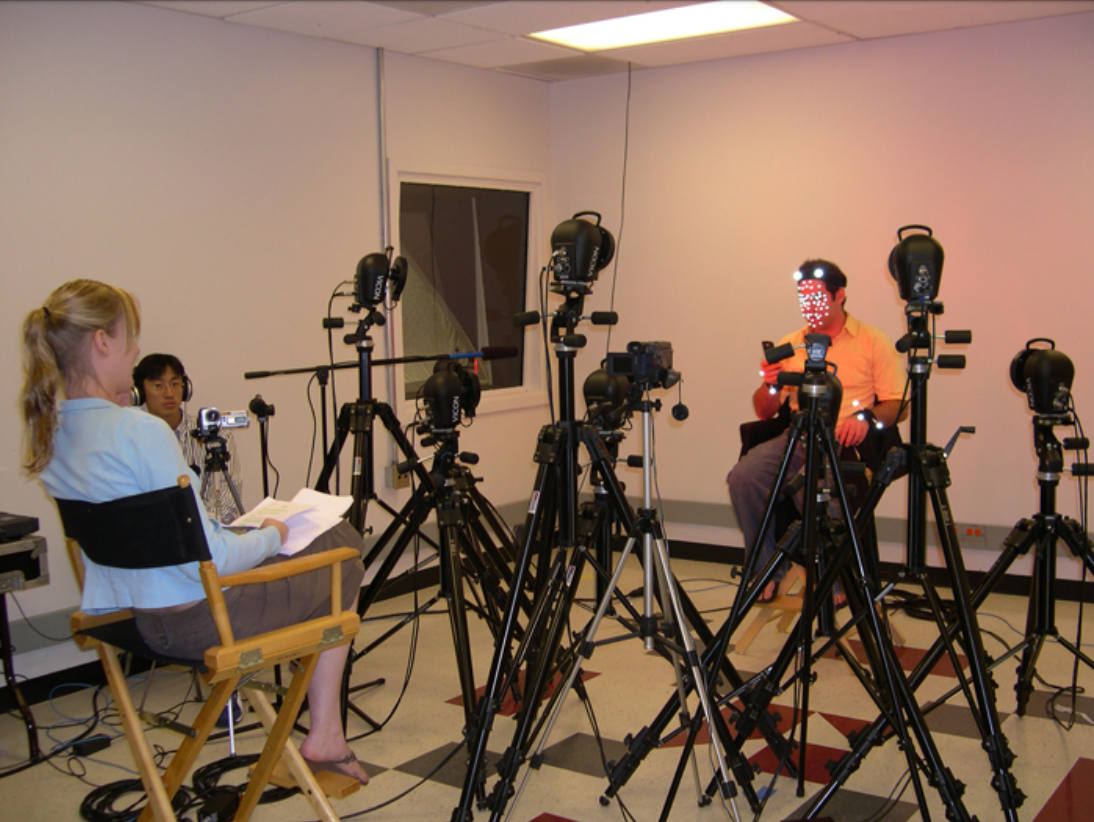
\includegraphics[width=0.9\textwidth]{Chapters/IEMOCAP_record.png}
\caption[A recording session of IEMOCAP database]{A recording session of IEMOCAP database}
\label{fig:data_recording}
\end{figure*}

Figure \ref{fig:data_recording} depicts the recording session of IEMOCAP dataset. As exhibited in the figure, the facial marker is used by only one of the participant. Thus, in this setting, we cannot use all 10039 utterances for audio-visual forecasting.  

% Chapter 2
\chapter{Feature Description} % Main chapter title
\label{Chapter2} % For referencing the chapter elsewhere, use \ref{Chapter1} 
\section{Speech Features}

On of the important modalities of expressing emotions are speech. Although the variations of speech is subjective, this is the most important human cues for recognizing human emotion. Research is done for which speech features are needed to be taken into account for emotion recognition. Most of the existing approaches to speech emotion recognition used acoustic features as classification input based on the acoustic correlation for emotion expressions. The most widely used speech or acoustic features are prosodic features e.g., pitch-related feature, energy-related features, and speech rate and spectral features e.g., Mel-Frequency Cepstral (MFCC) or filterbank features. Kwon and Lee reported that pitch and energy among these are strongest contributor in emotion recognition \cite{Kwon2003EmotionRB}. Neiburg et. al. used prosodic features (MFCC and pitch) to train a Gaussian Mixture Model classifier to recognize emotion \cite{Neiberg2006EmotionRI}. In this thesis, we use pitch, MFCC, MFB, and energy as speech features. The following sections will give a brief descrpition of those features. 

\subsection{Pitch}

The \textit{pitch} of the voice is one of the main characteristics. In the field of acoustic technologies it is also known as  \textit{fundamental frequency}. The period is know by the time taken by one vibratory cycle of the vocal folds. The frequency of vibration is, therefore, the number of periods per second, which is measured in Hertz.

\begin{equation}
    1\quad  Hertz\quad = \quad1\quad  vibration/second
\end{equation}

Now, in human ear, we perceive the pitch as the frequency of sound which means the higher the frequency, the higher we perceive the pitch to be and vice-versa. The fundamental frequency or pitch is directly related to the intonation. And the intonation is associated with expressive characteristics of the voice, which leads to express the emotion. 

However, estimation of the fundamental frequency is a complicated task. Of many different methods of detecting pitch, autocorrelation pitch detector is yet one of the most robust and reliable detectors of pitch \cite{pitch_rabi}. The autocorrelation computation works directly with the speech signal and thus the computation is fairly simple. Despite the requirement of  a high processing rate, a single multiplier and an accumulator is sufficient for the  hardware implementation. Moreover, the autocorrelation computation is not dependant on phase, making it robust in the case of usual phase distortions. However, there are several drawbacks associated with the use of this method. One of them is to determine which of several autocorrelation peaks due to the detailed formant structure corresponds to the pitch period. Next, the computation requires the window of computation of the short-time autocorrelation function. The window method creates two questions: first, there is the problem of choosing a perfect window size. Second, with the increase in autocorrelation index,  the effect of the window is to taper the autocorrelation function smoothly to zero. This effect tends to make the above difficulties more complex.  Another problem is the subjective difference in the analysis window.  For high-pitched speakers the analysis frame should be short (5-20 ms), and for low-pitched speakers it should be long (20-50 ms). 

Researchers demonstrated many different solutions to this problem. Most of these solutions used a sharp low-pass filter with cutoff frequency around 900 Hz. These solutions eliminates the effect of higher formant peaks. However, there are trade-offs to this method which includes elimination of all other higher formants, and results in loss of information. Another set of solutions suggest the flattening of speech signals for removal the first formant \cite{rabi_1, Sondhi}. The flattening is done by various methods, including center clipping and spectral equalization \cite{rabi_1}, inverse filtering, spectral flattening, and a Newton transformation \cite{markel}.

We discuss the autorrelation process of pitch estimation in brief. Let's assume the discrete time speech signal $x(n)$ which is defined for all $n$. We can describe the autorrelation function as:

\begin{align}
    {\phi__x} (m) = \lim_{N \to \infty} \frac{1}{2N + 1}\sum_{n=-N}^{N}x(n)x(n+m)
    \label{eqn:autocorr}
\end{align}


The function $\phi __x$ performs a noninvertible transformation of the signal. It is mainly useful for depicting the waveform structure. Now, if our input signal $x(n)$ is periodic with period P, we can write, 
\begin{align}
    \phi{__x} (m) = \phi{__x} (m+p)
    \label{eqn:periodic}
\end{align}


Equation \ref{eqn:periodic} indicates that autocorrelation is also periodic with the same period as the main signal. It can be written in other way: periodicity in the autocorrelation function can be inferred as periodicity in the signal as well. Now, speech is a non-stationary signal. Therefore, the long-term autocorrelation as described in equation \ref{eqn:autocorr} is not realistic. Hence, we present short-term autocorrelation function, and it is defined as:


\begin{align}
     \phi{__l} (m)  = \frac{1}{N} \sum_{n=0}^{N'-1}[x(n+l)w(n)][x(n+l+m)w(n+m)]
\end{align}

where, $0\leq m \leq {M__0}  -1$. Here, $w(n)$ is the appropriate window for analysis. $N$ is the
section length,  $N'$ is the number of signal
samples used in the computation of $\phi{__l} (m)$, $M__0$ is the autocorelation point amount, and $l$ denotes the index of the starting sample of the frame. In most research, the $N'$ is empirically set to, $N'= N- m $ so that only the N samples in the analysis frame.

% \begin{align}
% & i^\tau = \sigma(W_{xi} x^\tau + W_{hi} h^{\tau-1} + W_{ci} c^{\tau-1} + b^i) \\ 
% & F^\tau = \sigma(W_{xf} x^\tau + W_{hf} h^{\tau-1} + W_{cf} c^{\tau-1} + b^f) \\ 
% & \tilde{c}^{\tau} = tanh(W_{xc} x^{\tau} + W_{hc} h^{\tau-1} + b^c) \\ 
% & c^{\tau} = F^\tau * c^{\tau-1} + i^{\tau} * \tilde{c}^\tau\\
% & o^\tau = \sigma(W_{xo} x^\tau + W_{ho} h^{\tau-1} + W_{co} c^{\tau-1} + b^o) \\ 
% & h^\tau = o^\tau * tanh(c^\tau) 
% \end{align}


\subsection{Intensity}
\label{intensity}

Sound intensity is the power carried by sound waves per unit area in a direction right angle to that area. Speech intensity is one of the powerful entity through which emotion is expressed. Sound intensity $I$ is defined as,

\begin{align}
    \vec{I} = p\Vec{v}
\end{align}
 where, $p$ is the sound pressure and $\Vec{v}$ is the velocity of sound. As velocity and intensity both are vectors, they have magnitude and directions. The direction of sound intensity is the average direction of energy. Therefore, the average sound intensity can be written as,
 \begin{align}
    \vec{I} = \frac{1}{T}\int_{0}^{T} p(t)\vec{V}(t)dt
\end{align}
 
Now, for spherical propagation of sound at a radius $r$, intensity equation can be written as,

\begin{align}
    I(r) = \frac{P}{A(r)} = \frac{P}{4\pi r^2}
\end{align}

where, $P$ is the power of sound and $A(r)$ is the surface area of the sphere through which sound is propagating. 

The intensity of sound is also calculated with reference to a commonly used sound intensity. The unit of such measurement is decibel (dB).

\begin{align}
    sound\_ intensity\_ level = 10\log \frac{I}{I_0} dB
\end{align}

where, $I$ is the sound intensity and $I_0$ is the reference sound intensity.

\subsection{Mel-Frequency Cepstram}
\label{mfcc}

Sound is not interpreted by human auditory system in a linear scale. As the frequency is increased, the comprehension of pitch becomes logarithmic. Therefore, in cases like emotion, where human perception is more important than actual sound properties, mel-frequency cepstrum becomes significant. In speech signal  processing, the mel-frequency cepstrum (MFC) is a representation of the short-term power spectrum of a sound. MFCs are based on a linear cosine transform of a log power spectrum on a nonlinear mel scale of frequency. Mel-frequency cepstral coefficients (MFCCs) are coefficients that builds an MFC. In the mel-frequency cepstrum, frequency bands are equally spaced in mel-scale which has close relation to human ear perception. 

There are several steps involved in calculation the MFCC. First, we apply a pre-emphasis filter on the signal to amplify the high frequencies. A pre-emphasis filter is useful in balancing the frequency spectrum and improving the Signal--to--Noise Ratio (SNR). After that, signals are split into frames. Speech is a non-stationary signal and thus, its properties vary with time. Therefore, we need short frames to make a reasonable Fourier transform. In this way, we can obtain a better approximation of the frequency contours of the speech signal by concatenating adjacent frames.
\begin{figure*}
\centering
   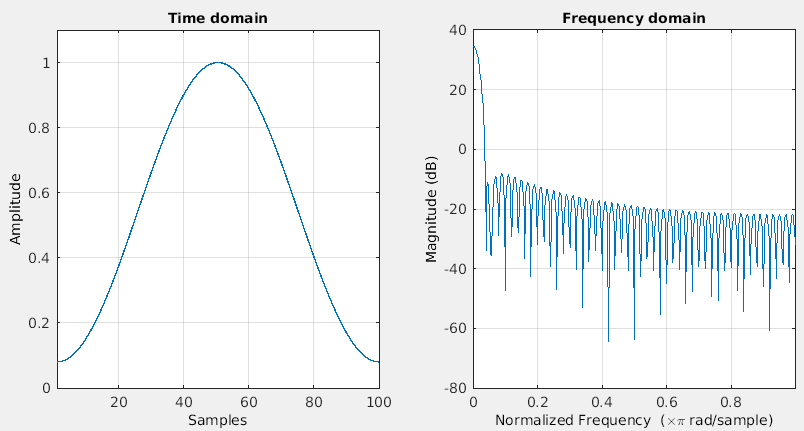
\includegraphics[width=0.9\textwidth]{Figures/Humming.png}
\caption[Humming Window]{A 100-sampling point Hamming window in time and frequency domain. }
\label{fig:humming}
\end{figure*}
After the framing step, we apply a hamming window function to those frame. Using a window function reduces the spectral leakage. The hamming window has the following form:
\begin{align}
    w[n] = 0.54 -.46 \cos{\frac{2\pi n}{N-1}}
\end{align}

where N is teh window length. A time and frequency domain representation is depicted in figure \ref{fig:humming} where 100 samples are used. 

Then, we perform a  N-point FFT on each windowed frame to calculate the frequency spectrum. This process is known as Short-Time Fourier-Transform (STFT), where N is empirically chosen as 256 or 512. The power spectrum is calculated using the equation: 
\begin{align}
    P = \frac{|FFT(x_i)|^2}{N}
\end{align}

Here, $x_i$ is the $i^{th}$ frame for speech signal $x$.  

At the final step, we compute filter banks by applying triangular filters on a mel-scale to the power spectrum to extract frequency bands. The following formula is used to convert the frequency scale to the mel-scale.
\begin{align}
    M(f) = 1125\ln({1 + \frac{f}{700}})
\end{align}

To convert back to frequency scale, 

\begin{align}
    M^{-1}(m) = 700(\exp{\frac{m}{1125}} -1)
\end{align}

The first filterbank will start at the first point, reach its peak at the second point, then return to zero at the 3rd point. The process goes on in the same way. The filterbank follows the criteria below:


\begin{align}

H_m (k) = \begin{cases} 
0, &  k \le f(m-1) \\ \frac{k-f(m-1)}{f(m)-f(m-1)}, & f(m-1)\leq k \leq f(m)\\\frac{f(m+1)-k}{f(m+1)-f(m)}, & f(m) \leq k \leq f(m+1)\\ 0, & k > f(m+1)
\end{cases}
\end{align}

Now the filter bank coefficients can be highly correlated, and such features can create instability in machine learning algorithm . Hence, we can apply Discrete Cosine Transform (DCT) to diminish the correlation of the filter bank coefficients and produce a compressed representation of the filter banks. This is how the MFCCs are obtained. 

\section{Facial Features}

Facial expressions are the most important modality to recognize emotion. The facial features are based on local spatial position or displacement of three-dimensional position of facial regions. Pantic et. al. provided a detailed review on facial features \cite{19}. Emotion recognition system from facial muscle movement was studied by Mase \cite{16}.  He used optical flow to detect the muscle movement in 11 facial regions. As classification algorithm, K-nearest neighbor rule was used, with an accuracy of 80\%. A similar research was conducted bt  Yacoob et. al. \cite{22}, where nstead of using facial muscle actions, they built a dictionary which converted motions associated with edge of the mouth, eyes and eyebrows, into a linguistic, perframe, mid-level representation. Their classification system used a rule-based approach with 88\% accuracy score. One of the major application of facial features involved Action Units (AU),  which is developed by Ekman and Friesen \cite{10}. For example, Tian et al. recognized the AUs using lip, nasolabial furrow and wrinkles \cite{21} . They located the shape and placement of those features by leveraging geometrical models with 96\% accuracy. Essa et al. quantified facial movements based on parametric models \cite{11}.


\begin{figure*}
\centering
   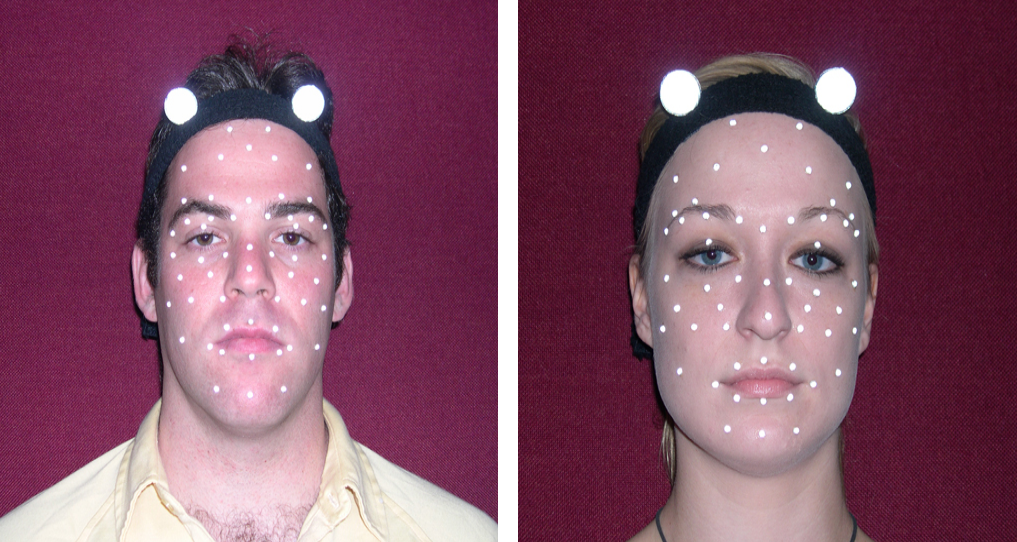
\includegraphics[width=0.9\textwidth]{Chapters/IEMOCAP_FACE.png}
\caption[The facial marker regions of IEMOCAP database]{The facial marker regions of IEMOCAP database }
\label{fig:IEMOCAP_FACE}
\end{figure*}



In the IEMOCAP database, the system is based on visual information, which is described in figure \ref{fig:IEMOCAP_FACE}. The spatial 3-D data collected from the motion capture markers in each frame of the video is transformed into a 4-dimensional feature vector per sentence. Those vectors are used as input to the classifier.  After the motion data are captured, they are normalized. First, all markers are translated in a  way that a nose marker be the local coordinate center of each video frame. Then, as  a reference frame, one frame with neutral and close-mouth head pose is selected. After that, three approximately rigid markers define a local coordinate origin for each frame. Next, a rotation of the coordinates are performed to align them with the reference frame. Each data frame has the following blocks of facial region : forehead, eyebrow, low eye, right cheek and left cheek area. For each block, a data vector is produced by a concatenation of the 3D coordinate positions. Then, Principal Component Analysis (PCA) based method is implemented to reduce the number of features per frame into a 10-dimensional vector for each area. Use of the PCA to feature reduction covers more than 99\% of the variation. 

\newpage
\chapter{Deep-Learning Architecture}

Deep learning (DL) has established a new era in the field of machine intelligence. With its effectiveness, DL is making tremendous impact  in areas, like disease diagnosis, precision medicine, self-driving cars, predictive forecasting, facial and speech recognition, and emotion recognition. For large datasets, one of the major and painstakingly tasks is building the handcrafted features in traditional machine learning algorithms. These algorithms are not scalable for large-sized data sets, resulting in poor performances.  Deep learning with human-like neuron representation contains several layers of units with highly optimized algorithms and structures. The nodes or units in the layers are connected to nodes in adjacent layers with some weight value. The computed values undergo a transformation based on the activation function, which can be sigmoid or ReLU. By performing the backpropagation, the layers rectify their errors and learns imitating human brain. 

The first prototype of Deep Learning was initiated by a perceptron \cite{Rosenblatt1958ThePA}. In that work, Rosenblatt used two layers of processing units that could detect simple patterns. However,  after a discovery of an MIT professor, suggesting the inefficiency of such network, neural network entered a dark phase \cite{Minsky1969PerceptronsA}.  Although proposed in 1975 by Werbose, the breakthrough of deep learning occured in 2015 after the revolutionary work by LeCun et. al. \cite{Deep_LEarning}.  

With deeper understanding of backpropagation, several variants of the network architecture was proposed and implemented, such as, FC, LSTM, BLSTM, CNN, GAN and many more \cite{g1,g2,g3,g4}. In this thesis, we used a FC, LSTM and BLSTM architecture. In the next subsection, these architectured will be discussed in brief. 

\section{Fully-Connected Neural Network}
\label{FC-DNN}

Fully-Connected deep learning frameworks are the most basic architecture of deep learning. By multiple connections, these networks learns the feature importance and produce result. 
\begin{figure*}
\centering
   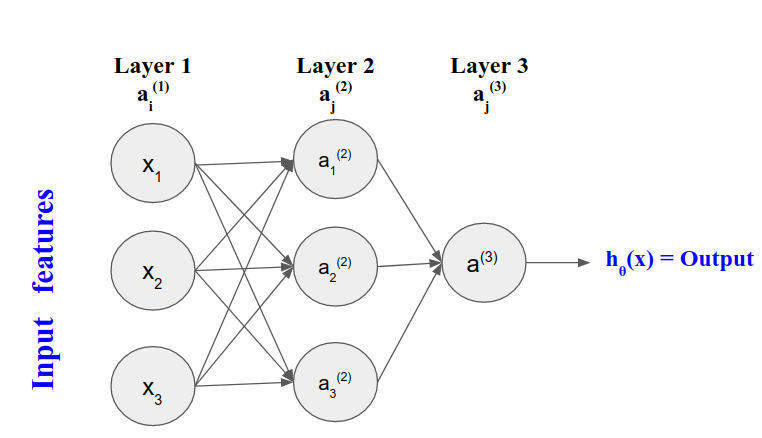
\includegraphics[width=0.9\textwidth]{Chapters/simple_NN.png}
\caption[A simple neural network]{A simple neural network }
\label{fig:simple_NN}
\end{figure*}

Let's assume that we have a dataset containing $n$ data-points with each of them having three input features $x_1, x_2, x_3$, and corresponding output $y_1, y_2, y_3$. If the dataset is large or complex enough, a simple logstic regression model will not be sufficient to map the complexity. Hence, we need a neural-network mapping for the representation of the features. 

In figure \ref{fig:simple_NN}, a simple neural network for such a task is presented. The first layer is input layer, which is defined as $a^{(1)}$. Then, the input is mapped to a hidden layer $a^{(2)}$ by some weights, from which we go to a final layer. The final layer simply transforms the output into our desired representation. Based on a backward propagation algorithm, the network learns from its errors. Therefore, we need to discuss the steps of backpropagation in detail. 

Backpropagation is defined as an algorithm to calculate the gradient which is needed to adjust the weights of the neural network. First indrouced in 1970 \cite{linnainmaa1970representation}, the backpropagation algorithm is brought into light by Rumelhart et. al. in 1986 \cite{Bacprop_hinton}. The algorithm is based on the partial derivative of the objective function with different weight parameters, which demonstrated how fast the change of objective function occurs with change in weight. 

Neural network also uses activation functions. There are many choices of activation function, but popular choices include sigmoid and ReLU. A detailed representation of the activation functions are presented in figure \ref{actfn}.
\begin{figure}
\centering
\begin{subfigure}{0.4\linewidth}
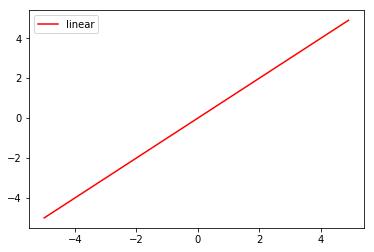
\includegraphics[width=\linewidth]{Figures/linear_act.png}
%\vspace{-0.3cm}	
\label{linear} 
\caption{Linear}
\end{subfigure}
%\vspace{0.1cm}
\begin{subfigure}{0.4\linewidth}
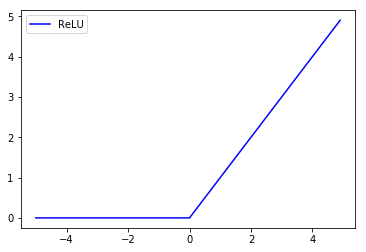
\includegraphics[width=\linewidth]{Figures/relu_act.png}
%\vspace{-0.3cm}
	\label{relu}
          \caption{ReLU}
\end{subfigure}
\\
%\vspace{0.1cm}
\begin{subfigure}{0.4\linewidth}
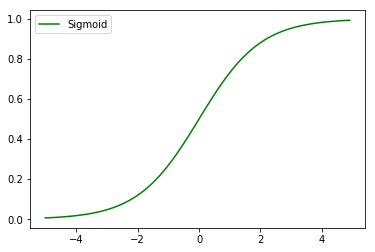
\includegraphics[width=\linewidth]{Figures/sigmoid_act.png}
%\vspace{-0.3cm}
	\label{sig}
          \caption{Sigmoid}
\end{subfigure}
\begin{subfigure}{0.4\linewidth}
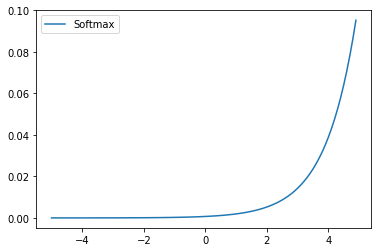
\includegraphics[width=\linewidth]{Figures/softmax_act.png}
%\vspace{-0.3cm}
	\label{soft}
          \caption{Softmax}
\end{subfigure}
\caption{NN Activation functions.}
\label{actfn}
%\vspace{-15pt}
\end{figure}

We can derive the equation for different units in layer 2 from figure \ref{fig:simple_NN}.

\begin{align}
    {a_1}^{(2)} = g(\theta _{10}^{(1)}x_{0} + \theta _{11}^{(1)}x_{1} + \theta _{12}^{(1)}x_{2} +\theta _{13}^{(1)}x_{3}) \\
    {a_2}^{(2)} = g(\theta _{20}^{(1)}x_{0} + \theta _{21}^{(1)}x_{1} + \theta _{22}^{(1)}x_{2} +\theta _{23}^{(1)}x_{3}) \\
    {a_3}^{(2)} = g(\theta _{30}^{(1)}x_{0} + \theta _{31}^{(1)}x_{1} + \theta _{32}^{(1)}x_{2} +\theta _{33}^{(1)}x_{3}) \\
    h_{\theta}(x) = a_{1}^{(3)} = g(\theta _{10}^{(2)}a_{0}^{(2)} +\theta _{11}^{(2)}a_{1}^{(2)} + \theta _{12}^{(2)}a_{2}^{(2)} +\theta _{13}^{(2)}a_{3}^{(2)})
\end{align}


In the above set of equations, the term $\theta$ with different subscript and superscript denotes the weight associated from units of one layer to the units of the other. $x_0$ and $a_0$ are the bias term. The term $a_i^{(j)}$ is denoted as $i^th$ unit in $j_th$ layer. The function $g(.)$ represents the activation function. This is called the \textit{forward propagation}(FP). If we consider the layers as vectors, we can write the FP equation set as follows:

\begin{align}
    %Forward &\quad Propagation\\
    a^{(1)} &= x \\
    z^{(2)} &= \theta^{(1)}a^{(1)} \\
    a^{(2)} &= g(z^{(2)}) \\
    z^{(3)} &= \theta^{(2)}a^{(2)}\\
    a^{(3)} &= g(z^{(3)})\\
    z^{(4)} &= \theta^{(3)}a^{(3)}\\
    a^{(4)} &= h_{\theta}(x)=g(z^{(3)})
\end{align}



Now, at initial stage, only the network architecture is defined and thus, the weights are randomized. Therefore, there will be error term and we represent the error in an objective function (also known as \textit{cost function}). 

If the dataset has $m$ number of point and $K$ number of classes to classify, we can write the objective function as:

\begin{align}
    J(\theta) = - \frac{1}{m}[\sum_{i=1}^{m}\sum_{k=1}^{K}y_{k}^{(i)}log(h_{\theta}(x^{(i)}))_{k}+ (1-y_{k}^{(i)})log(1-h_{\theta}(x^{(i)}))_{k})]
    \label{eq:cost}
\end{align}


As evident from equation \ref{eq:cost}, the cost function $J(\theta)$ is the function of weightparameter $\theta$. Therefore, our target is to find such a group of weights, $\theta$, that will minimize $J(\theta)$. We will introduce an error term $\delta$, which we can obtain by the partial differentiation of the objective function with respect to $\theta$. By chain differentiation, it can be shown that, 
\begin{align}
    \frac{\partial J(\theta)}{\partial \theta_{ij}^{(l)}} = a_{j}^{(l)} \delta_{i}^{(l+1)}
\end{align}

We can calculate the error term for each node or unit. $\delta_{j}^l$ represents the error of unit $j$ in layer $l$. 
%set $\Delta_{ij}^l=0$\



\begin{algorithm}[H]
\SetAlgoLined
\KwResult{Partial derivation for each parameter. Vector $D^{(l)}$}
 set $\Delta_{ij}^l=0$\;
 set $i=1$\;
 \While{$i \leq m$}{
  instructions\;
  Perform forward propagation to compute $a^l$ for each layer\;
  Compute the error term $\delta$\;
  \eIf{this is final layer}{
  $\delta^{l=L}=a^{L}-y^{i}$\;
  }{
  $\delta^{l}=\theta^{l}\delta^{(l+1)}\cdot(a^{l}\cdot(1-a^{l}))$\;
  }
  
 Update $\Delta$,\;
 $\Delta_{ij}^{(l)}:=\Delta_{ij}^{(l)} + a_{j}^{(l)} \delta_{i}^{(l+1)}$\;

 }

 $D^{(l)}=\frac{1}{m}\Delta^{(l)}$\;

 \caption{Backpropagation algorithm}
\end{algorithm}
\vspace{+1cm}
In our EF problem, we use a FC network with four layers and 256 units per layer, and ReLU is used as activation function. The final layer is softmax with four units. 

\section{Recurrent Neural Network (RNN)}
\label{RNN}
Recurrent neural networks have the ability to comprehend sequential data. One of the major drawbacks of FC networks is, features are mapped into a representation without consideration of their interdependence. RNN provides an architecture to solve this problem. 

\begin{figure*}
\centering
   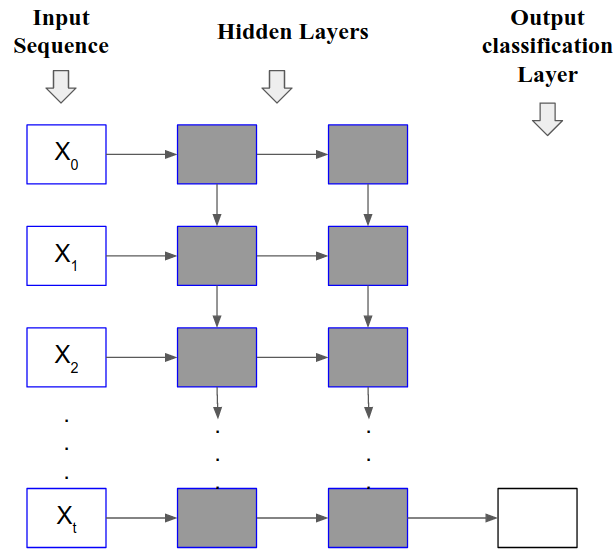
\includegraphics[width=0.5\textwidth]{Chapters/RNN.png}
\caption[A many-to-one RNN architecture]{A many-to-one RNN architecture }
\label{fig:RNN}
\end{figure*}

In figure \ref{fig:RNN}, a many-to-one RNN architecture is shown. RNN takes a series as features. Then inside the hidden layer, the hidden units can be thought of as multiple copies of the same network, each passing a message to a successor. Of many variants of RNN, Long Short-Term Memory (LSTM) network and Bidirectional Long Short-Term Memory (BLSTM) networks are the most popular one. The detail of these networks are explained in the next section.

\subsection{Long Short-Term Memory Network (LSTM)}
\label{LSTM}

The LSTM network is an enhanced version of the RNN that has the added advantage of handling the vanishing gradient problem \cite{LSTM}. An LSTM layer is composed of recurrently connected memory blocks, where the memory cells have three gate units: the input, output, and forget gates. Briefly, the cell input is multiplied by the activation of the input gate, the cell output by that of the output gate, and
the previous cell values by the forget gate \cite{Meta}. Thus, information is retained and stored over an extensive time period. For BLSTM, the network is composed of both the forward and backward directions of LSTM. 

\begin{figure*}
\centering
   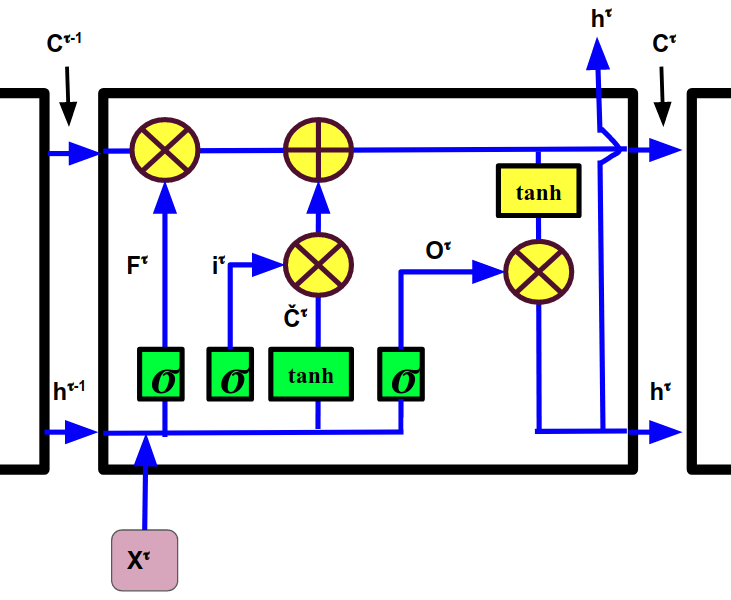
\includegraphics[width=0.6\textwidth]{Chapters/cell_LSTM.png}
\caption[The basic cell structure of LSTM]{The basic cell structure of LSTM }
\label{fig:LSTM}
\end{figure*}


The internal cell state of an LSTM network ($c^{\tau}$) at time $\tau$ is computed based on the current input ($x^{\tau}$) and the previous cell state ($c^{\tau-1}$).
The combination of input ($i^{\tau}$) and forget ($F^{\tau}$) gates control how much the previous cell state $c^{\tau-1}$ and the current input $x^{\tau}$ contribute to the current cell state $c^{\tau}$.
The activation function for both forget and input gates is a sigmoid function ($\sigma$) that outputs values between 0 and 1. The current cell state  $c_\tau$ is determined by the following equations: 
\begin{align}
& i^\tau = \sigma(W_{xi} x^\tau + W_{hi} h^{\tau-1} + W_{ci} c^{\tau-1} + b^i) \\ 
& F^\tau = \sigma(W_{xf} x^\tau + W_{hf} h^{\tau-1} + W_{cf} c^{\tau-1} + b^f) \\ 
& \tilde{c}^{\tau} = tanh(W_{xc} x^{\tau} + W_{hc} h^{\tau-1} + b^c) \\ 
& c^{\tau} = F^\tau * c^{\tau-1} + i^{\tau} * \tilde{c}^\tau\\
& o^\tau = \sigma(W_{xo} x^\tau + W_{ho} h^{\tau-1} + W_{co} c^{\tau-1} + b^o) \\ 
& h^\tau = o^\tau * tanh(c^\tau) 
\end{align}
where $o^\tau$ is the output gate that determines the contribution of  current cell state $c^\tau$ to the current output $h^\tau$. We can also rewrite $h^\tau$ and $c^\tau$ as follows:
\[
(h^\tau, c^\tau) = \mathcal{G}(x^\tau, h^{\tau-1}, c^{\tau-1})
\]
where $\mathcal{G}$ is the LSTM activation function. 


\subsection{Bidirectional Long Short-Term Memory Network (BLSTM)}
\label{BLSTM}
\begin{figure*}
\centering
   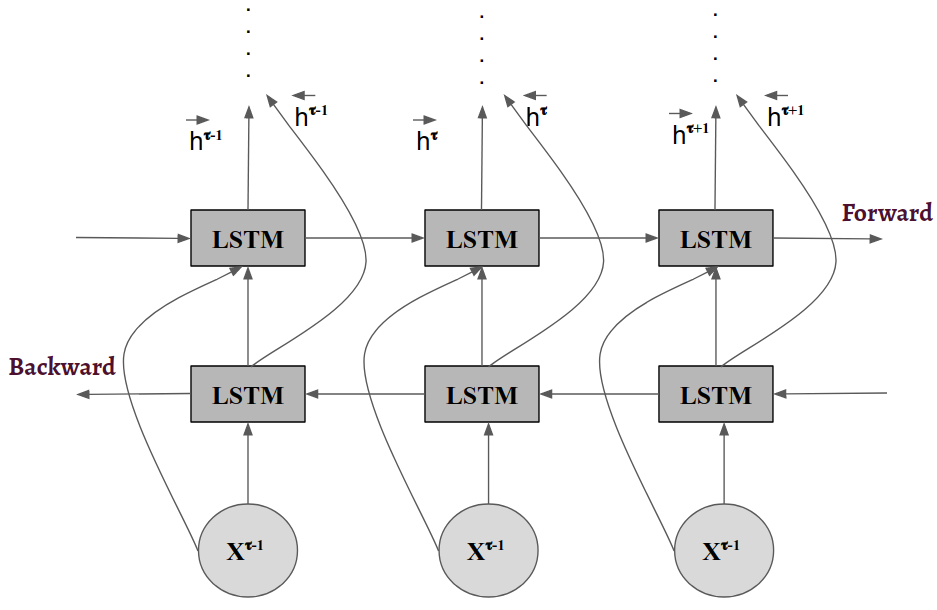
\includegraphics[width=0.6\textwidth]{Chapters/BLSTM.png}
\caption[Architecture of BLSTM]{Architecture of BLSTM }
\label{fig:LSTM}
\end{figure*}

To process the input sequence in both forward and backward directions, the bidirectional LSTM (BLSTM) is used to capture the dynamics in both past and future samples.
For BLSTM, $h^\tau$ will be composed of both the forward and backward directions, $h^\tau = [\overrightarrow{h^\tau}; \overleftarrow{h^\tau}]$ and it is defined as follows:
\begin{align}
& (\overrightarrow{h}^\tau, \overrightarrow{c}^\tau) = \overrightarrow{\mathcal{G}}(x^\tau, \overrightarrow{h}^{\tau-1}, \overrightarrow{c}^{\tau-1}) \\
& (\overleftarrow{h}^\tau, \overleftarrow{c}^\tau) = \overleftarrow{\mathcal{G}}(x^\tau, \overleftarrow{h}^{\tau-1}, \overleftarrow{c}^{\tau-1})
\end{align}

Our main architecture will contain deep LSTM (D-LSTM) / BLSTM (D-BLSTM) networks, followed by a FC-DNN. 


\newpage
\chapter{Methodology}
\label{methodology}

\section{Feature Extraction and Data Processing}
Following the work of Metallinou et al. \cite{Meta}, both the audio and visual data were extracted at the same frame rate of 25 ms and the window of 50 ms. 

For the audio data, we extract pitch, energy, 12 Mel Frequency Cepstral Coefficients (MFCC) and 27 Mel Filter Bank (MFB) coefficients, and we use Praat for  feature extraction \cite{praat}.  The 46 total 3-D markers allow for 138-dimensional facial landmark representation. We use linear interpolation method to remove the NaN values. If the total amount of NaN values in an utterance is greater than 30\% of total frames, we exclude the utterance. Additionally, we exclude utterances with the audio data that has zero pitch in all frames since these utterances do not contain meaningful audio information.

We use utterance-level statistical features, namely, mean, standard deviation, first quantile, third quantile, and inter-quartile range. Therefore, building in the 179 frame-level features (41 audio and 138 facial landmark features), we have 895 statistical features in total. The features are normalized speaker-wise using z-normalization. D-LSTM and D-BLSTM use  window-level features. The windows are made by taking statistical features over 30 frames  with a 50\% overlap. As the IEMOCAP utterances have different length, we use zero-pad and later used a masking layer \cite{keras}. All the experiments were done using Keras \cite{keras}. 

\section{Emotion Forecasting Methods}
We analyze emotion forecasting based on the forecasting windows and presence of previous history utterance in forecasting.
\subsection{Forecasting Windows}
Due to the difference of length in various utterances of IEMOCAP database, we present two approaches of forecasting windows. The utterance forecasting will consider only the speaking turns after which forecasting will be done, while the time forecasting will consider the time amount for forecasting.
\subsubsection{Utterance Forecasting (UF)}
\label{utt_steps}
For forecasting with utterance steps, we consider the emotional flow of one participant in a dialog only. For 1 utterance forecasting (UF 1), we choose the data of the present utterance and the label for the next utterance of the same speaker in the same dialog. Similarly, for $k$-utterance forecasting (UF $k$), the data will come from current utterance and the label will come from the utterance of $n$ future steps.  

To illustrate, let $L$ be the set of all utterance labels of a particular speaker $A$, and $U$ be the set of all utterance feature data of $A$. If $A$ has $n$ number of utterances, then
$L=\{L_1,L_2,L_3...L_n\}$, 
and
\[
U=\{Utt_{1}^A, Utt_{2}^A, Utt_{3}^A...Utt_{n}^A\}
\]
 where $L_x$ is the label of  utterance $Utt_{x}^A$, where $x=1,2,3...n$.

 As in IEMOCAP, a dialog contains a complete scenario of emotional conversation, the forecasting has to be done within a dialog.    For instance,  the mapping of feature data  to the labels for a $k$ utterance forecasting will be $Utt_{1}^A \rightarrow L_{1+k}$ and so on. If the dialog has $d$ number of utterances, then for the $dth$ utterance, $Utt_{d}^A$, we cannot have the $L_{d+k}$ labels. If $k>1$, we will have more utterances in every dialog which have no labels and  hence, must be discarded. Hence, the number of the utterances decreases in utterance forecasting (UF) 1, 2, and 3, as stated later in this section. 

\begin{figure}
\centering
   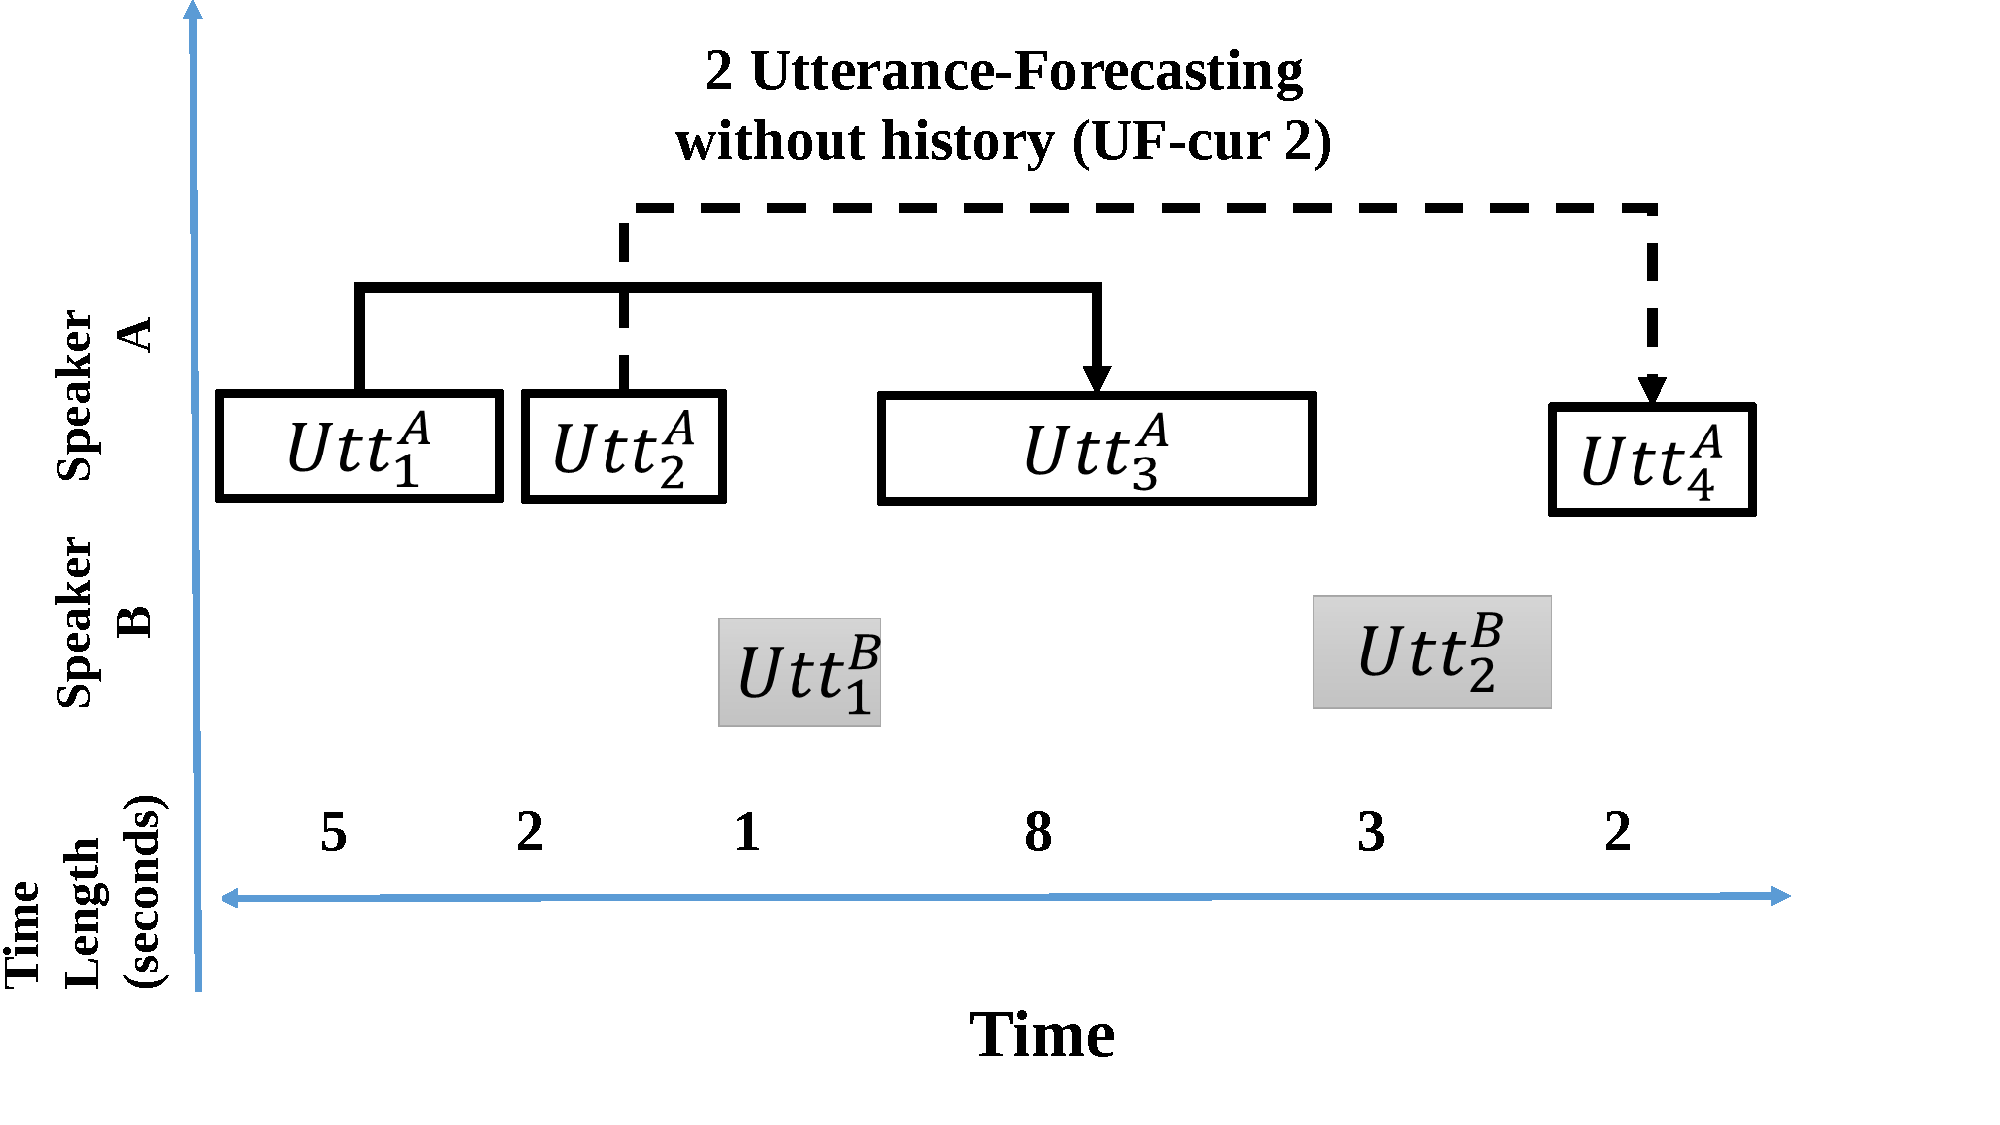
\includegraphics[width=0.6\linewidth]{Chapters/cur.pdf}
\caption[An example of emotion forecasting without history]{An example of emotion forecasting without history. Here, the data of $Utt_{1}^A$ will be used to forecast the emotion of the utterance $Utt_{3}^A$ .}
% \vspace{-0.3cm}
\label{fig:historyless}
\end{figure}

The process is described in Fig. \ref{fig:historyless}, which depicts the dataset re-processing for UF 2. If in a dialog, the conversation alternate between  speaker A and speaker B: $A \rightarrow B \rightarrow A \rightarrow B \rightarrow A$, then the utterance $Utt_{3}^A$'s label would be used for the data of utterance $Utt_{1}^A$. UF 1, 2, and 3 holds 2823, 2734, and 2662 utterances consecutively. These utterances have a mean time-distance (explained in the next section) of $4.71\pm5.37$ seconds $12.78 \pm8.55$ seconds and $21.48\pm10.78$  seconds, respectively. Note that, for utterance $Utt_{1}^A$, the forecasting label has to pass one utterance of the other speaker (B), while utterance $Utt_{2}^A$ has to pass two utterances of the other speaker. This creates inconsistency in the dataset and results in a large standard deviation of time-distance among the steps.


\subsubsection{Time Forecasting (TF)}
\label{time_grps}
Due to the inconsistency explained in previous section, we introduce  the \textit{time-distance} through which future emotion will be forecasted. Time-distance is defined as the time length from the current utterance to the forecasted utterance's emotional label for UF 1, 2 or 3 . Additionally, to calculate the time-distance, we also consider the length of the other speaker's utterance that falls in between the utterances of the same speaker. The calculation of time-distance starts from the middle point of the current utterance and ends at the middle point of the target utterance whose emotion is to be forecasted.

We divide the time-distances into several groups of 5-seconds range. TF 1 will have a forecasting time-distance of 3 second to 8 seconds, TF 2 will have a  time-distance length of 8 seconds to 13 seconds, and TF 3 will have a time-distance of 13 seconds to 18 seconds.  For example, in Fig. 1, the first forecasting will have a time-distance of 9.5 seconds $(2.5+2+1+4)$, and the second forecasting will have a time-distance of 14 seconds $(1+1+8+3+1)$. Therefore, although in terms of the forecasting window of UF, they will fall into same UF 2, in terms of TF, the first one will be part of TF 2 and the second one will be a part of TF 3.  For TF 1, 2 and 3, we have 1800, 1790, and 1725 utterances. The mean time-distance for TF 1, 2 and 3 are $5.56\pm1.36$ seconds, $10.40\pm1.43$ seconds, and $15.37\pm1.42$ seconds. 

It can be mentioned that we also experiment with longer step UF and TF. As the steps increase, the number of the utterances decrease and the average time-distances increase. Moreover, we also observe a gradual drop in the performances and hence, we stick to the step three for both UF and TF. 


\subsection{Absence or Presence of Previous History}
\subsubsection{History-Less Emotion Forecasting}
In the history-less technique, we experiment emotion forecasting using the current audio-visual data only with both forecasting windows, UF and TF. 
\subsubsection{History-Added Emotion Forecasting}
\label{history}
In this technique, in addition to the present emotional data, the prior utterance's data will also be used to forecast future emotion. An example is illustrated in Fig.\ref{fig:history}, where for 2 utterance forecasting (UF 2), along with the current utterance $Utt_{2}^A$, the previous utterance $Utt_{1}^A$ is also taken into account and the features are concatenated. For instance, considering the illustration of Section \ref{utt_steps}, for a $k$ utterance forecasting, the data will be,
\[
U=\{Utt_{1}^A, Utt_{1,2}^A, Utt_{2,3}^A...Utt_{n-k-1,n-k}^A\}
\]
and the labels will be
$L=\{L_{1+k},L_{2+k}...L_n\}$

where \[Utt_{n-k-1,n-k}^A=concatenation(Utt_{n-k-1}^A, Utt_{n-k}^A)\]
We conduct the history-added emotion forecasting using UF-his and TF-his approaches.
\begin{figure}
\centering
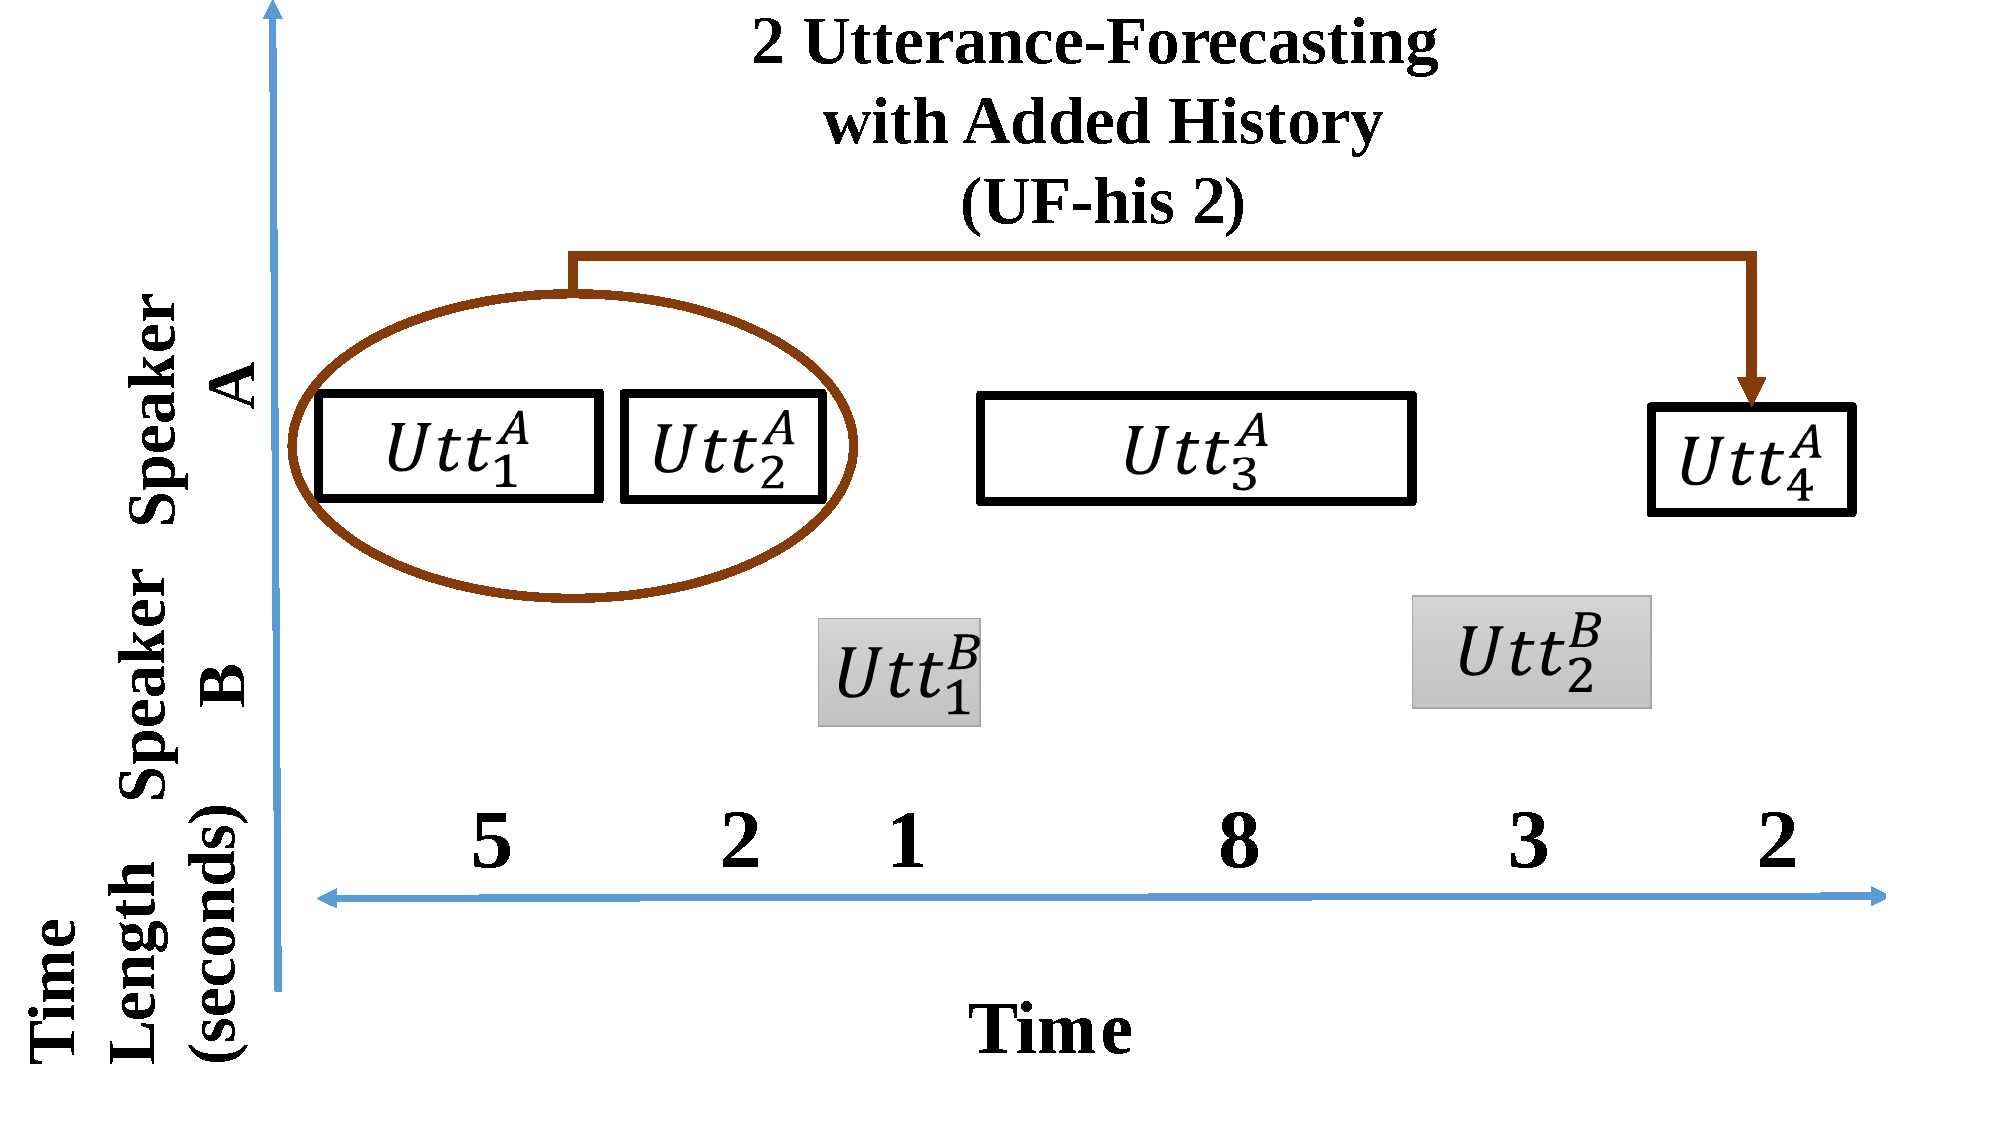
\includegraphics[width=.6\linewidth]{Chapters/his.pdf}
\caption[An example of emotion forecasting with added history from the previous utterance]{An example of emotion forecasting with added history from the previous utterance. Here to forecast the emotion of $Utt_{4}^A$ , the data of both $Utt_{1}^A$ and $Utt_{2}^A$  are used.  }
% \vspace{-0.75cm}
\label{fig:history}
\end{figure}
% \vspace{-.25cm}

\newpage
 \section{Experimental Setup }
Our FC-DNN model contains three fully connected layers with 256 memory units and one output softmax layer.  The D-LSTM uses two LSTM layers with 128 memory units each. After that, an FC layer is used with RELU as activation and finally a softmax output layer is stacked with the network. The D-BLSTM is built up with similar architecture with the LSTM layers having 128 memory units in both direction.   For all FC-DNN, D-LSTM and D-BLSTM, a rectified linear unit (RELU) is used as the activation unit. We use a learning rate of 0.0001 with the adam \cite{adam} optimizer and a batch size of 128. We also use an early stopping criteria, where the training stops if the validation accuracy does not improve after ten consecutive epochs. 

To measure the performance, we calculate the Unweighted (Average) Recall (UAR), which is defined as the mean recall of all the emotion classes over the ten test speakers. We perform leave-one-speaker-out cross-validation. The validation accuracy is used for choosing the number of epochs for early stopping. As suggested in previous research \cite{significance} , for testing the significance level of difference between different approaches, we use a paired t-test over ten speakers. We claim significance when $p$\textless$0.05$.


\newpage
\chapter{Results and Discussion}
\label{result_and_discuss}

As stated in Section \ref{approach}, we  use the UF-cur and TF-cur approaches for addressing \textbf{H1} and UF-his and TF-his for addressing \textbf{H2}. 


\section{History-Less Emotion Forecasting}

Table \ref{tab:history-less} summarizes the results of UF-cur and TF-cur experiments. For UF-cur 1, 2, and 3, the results support  \textbf{H1}. Although not statistically significant ($p$\textgreater$0.05$) , we achieve 0.97\%, 1.28\%, and 1.59\% improvement using D-LSTM over FC-DNN, while we observe  0.97\%, 1.91\%, and 0.85\% improvement using D-BLSTM. Nevertheless, we achieve a better set of accuracy with D-BLSTM than FC-DNN, it does not seem to work better than D-LSTM, particularly UF-cur 3. This may indicate that, as D-BLSTM has more complex modeling process than D-LSTM and it needs a large amount of data as well, our data quantity may be insufficient (2662 utterances for UF 3) for that purpose.

\begin{table}[h]
\centering
\caption{UAR(\%) comparison between static (FC-DNN)  and dynamic  (D-LSTM and D-BLSTM) models for both UF-cur and TF-cur approaches. The sign ``[*]'' denotes that the model is statistically significant ($p$\textless$0.05$) compared to the FC-DNN}
\begin{tabular}{l  l  l  l}
\hline

\makecell{\textbf{Forecasting}\\\textbf{Window}} & \makecell{\textbf{FC-DNN}\\} &  \makecell{\textbf{D-LSTM}\\} & \makecell{\textbf{D-BLSTM}\\} \\
\hline
\hline
UF-cur 1 & 57.96 & 58.93 & 58.95 \\

UF-cur 2 & 54.45 & 55.73 & 56.36\\      

UF-cur 3 & 51.40 & 52.99 & 52.25\\
\hline
TF-cur 1 & 57.05 & 57.37 & 57.81 \\

TF-cur 2 & 55.29 & 56.02 & 56.48\\      

TF-cur 3 & 52.93 & 55.35[*] & 55.53[*]\\
\hline
\end{tabular}
\label{tab:history-less}
\end{table}

 Table \ref{tab:history-less} also shows the performance comparison for TF-cur 1, 2, and 3. It shows that D-LSTM performs better than the FC-DNN model by  0.32\%, 0.73\%, and 2.42\% ($p$\textless$0.05$) for TF-cur 1, 2 and 3 respectively. When we consider both forward and backward dynamics by taking into account a bidirectional temporal model (D-BLSTM), we find better accuracy than FC-DNN model by 0.76\%, 1.19\%, and 1.60\% ($p$\textless$0.05$) respectively.  Therefore, the above experiments supports our hypothesis \textbf{H1} that temporal model can perform better than the static model.




\section{History-Added Emotion Forecasting}
As stated previously, adding history to present information incorporates more temporal contexts, which can result in an enhanced forecasting performance. Table \ref{table:history} describes the results of both UF and TF approaches with the history of previous utterance added.  Adding history improved the D-LSTM accuracy for UF-his 1, 2, and 3 by 1.75\%, 0.78\%, and 0.34\% compared to UF-cur D-LSTM approaches. We observe even more improvement in D-BLSTM performance. D-BLSTM  is improved by 2.38\% ($p$\textless$0.05$), 2.01\%, and 2.39\% ($p$\textless$0.05$) for UF-his 1, 2, and 3. 

For the TF-his approach, both the D-LSTM and D-BLSTM performance improves over the history-less performance. We observe an  improvement of 1.64\%, 2.25\% ($p$\textless$0.05$), and 2.37\% ($p$\textless$0.05$) for D-LSTM and 1.52\%, 1.95\%, and 2.87\% ($p$\textless$0.05$) for D-BLSTM in TF-his 1, 2, and 3 than the TF-cur approaches. Moreover, Table \ref{table:history} shows that in every case, unlike UF-cur result, the D-BLSTM outperforms D-LSTM performance. This may imply that D-BLSTM can process the information in a better way when adequate history is provided. 

\begin{table}[h]
\centering
\caption{Results of emotion forecasting with added history information: performance of UF-his and TF-his with dynamic modeling. The sign ``[*]'' denotes that the model with history-added technique is statistically significant ($p$\textless$0.05$) compared to the history-less technique of the model. }

\begin{tabular}{llll}
\hline
\makecell{\textbf{Forecasting}\\\textbf{Window}}  & \textbf{D-LSTM} & \textbf{D-BLSTM }\\
\hline
\hline
UF-his 1 & 60.68 & 61.33 [*] \\

UF-his 2 & 56.51 & 58.37 \\

UF-his 3 & 53.33 & 54.64 [*] \\

\hline

TF-his 1 & 59.01 & 59.33 \\

TF-his 2 & 58.27[*] & 58.43 \\

TF-his 3 & 56.72[*] & 58.40[*] \\

\hline
\end{tabular}
\label{table:history}
\end{table}



Furthermore, instead of previous utterance, we add a randomly chosen utterance of the same speaker (i.e., UF-random and TF-random) to compare the effect of adding random data with current utterance rather than the history.  Table \ref{table:noise} shows that for every case, compared to UF-random or TF-random, UF-his and TF-his performs significantly better ($p$\textless$0.05$). The UF-his 1, 2, and 3 has an improvement of 5.58\%, 4.50\%, and 4.65\% respectively with D-LSTM and 4.69\%, 5.64\%, and 5.30\% respectively with D-BLSTM. Similarly, for TF-his 1, 2, and 3, the improvement is 3.97\%, 5.83\%, and 5.71\% respectively with D-LSTM and 4.31\%, 6.13\%, and 7.53\% respectively with D-BLSTM, comparing with the randomly added data.  As adding random utterance in the data may harm the emotional temporal flow, we observe a diminished UAR performance. It implies that our improvement in history-added D-BLSTM performance is not merely coming from adding extra information, rather, by taking the proper history context into account. Therefore, we show that adding history information from one previous utterance can add an emotional context for the network to see the temporal flow pattern of the utterances and predict the future emotion, and hence, the results support \textbf{H2}. 

The reason for D-BLSTM network's superior performance in both UF-his and TF-his experiments may be that, as a more complex modeling framework compared to the D-LSTM,  the D-BLSTM model can see both past and future information. Thus, by achieving the history information, it can achieve substantial information by moving in both directions. 



\begin{figure*}
\centering
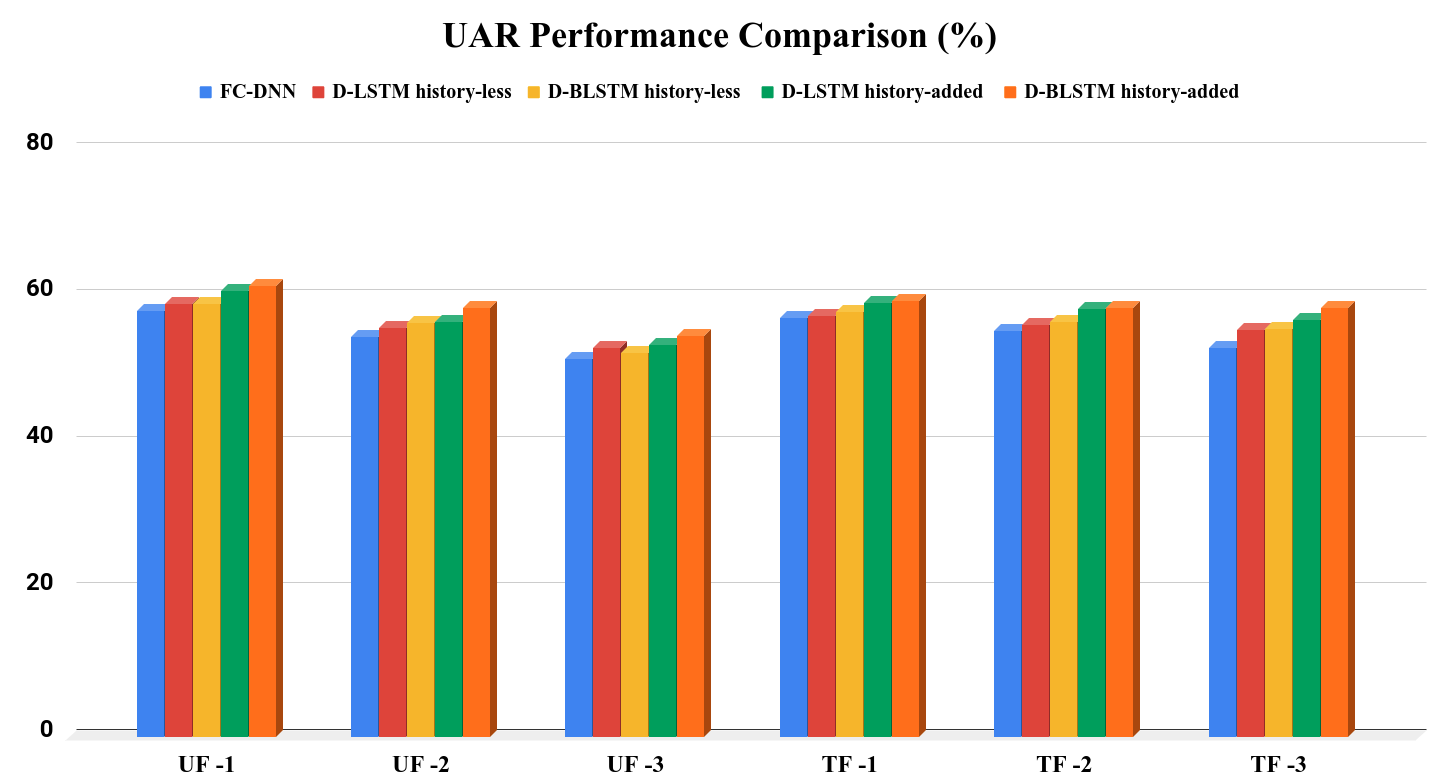
\includegraphics[width=.8\linewidth]{Chapters/compare.png}
\caption[Comparison of performance using different forecasting windows, and deep-learning framework]{Comparison of performance using different forecasting windows, and deep-learning framework.}
% \vspace{-0.75cm}
\label{fig:compare}
\end{figure*}

%%%new style
\begin{table}[h]
\centering
\caption{ UAR (\%) comparison of UF-his/TF-his with UF-random/TF-random. The sign ``[*]'' denotes the  statistically  significant ($p$\textless$0.05$) result of history added technique, compared to the randomly added data. }
\begin{tabular}{llll}
\hline
\makecell{\textbf{Forecasting}\\\textbf{Window}}  & \textbf{D-LSTM} & \textbf{D-BLSTM}\\
\hline
\hline
UF-his 1 & 60.68 [*] & 61.33 [*] \\
UF-random 1 & 55.10 & 56.62 \\
\hline
UF-his 2 & 56.51 [*] & 58.37 [*] \\
UF-random 2 & 52.01 & 52.73 \\
\hline
UF-his 3 & 53.33 [*] & 54.64 [*] \\
UF-random 3 & 48.68 & 49.34 \\
\hline
\hline
TF-his 1 & 59.01 [*] & 59.33 [*] \\
TF-random 1 & 55.04 & 55.02 \\
\hline
TF-his 2 & 58.27 [*] & 58.43 [*] \\
TF-random 2 & 52.44 & 52.30 \\
\hline
TF-his 3 & 56.72  [*] & 58.40 [*] \\
TF-random 3 & 51.01 & 51.97 \\
\hline
\end{tabular}
\label{table:noise}
\end{table}




\section{Further Analysis}
We further investigate the performance of utterances that have the same target forecasting and current emotion labels. We examine whether the performance of emotion forecasting is biased toward that of emotion recognition. We define the term \textit{same-label} as, for any forecasting approach, the ratio of instances, where forecasting and recognition ground truths are same, to all the forecasting ground truth labels. We find that in all forecasting approaches, more than two-third of the forecasting utterances have the same ground truth labels with the recognition. We analyzed the emotion specific performances of such case. For example, for UF-cur 3, we observe the highest UAR with the `Happy' emotion (83.25\%), and the lowest with the `Neutral' emotion (36.55\%). However, When the forecasting label is different from current emotion label, we achieve lower UAR as expected. For instance, UF-cur 3 D-BLSTM results achieve up to 36.72\% for angry, 41.30\% for happy, 17.09\% for neutral, and 32.10\% for sad classes. Hence, the results imply that the training and testing data used for the forecasting experiments may be biased towards the current emotion labels. Therefore, an extensive analysis on forecasting window is needed to develop a more robust emotion forecasting system. 

\begin{table}[h]
\centering
\caption{The ratio of identical labels of forecasting and recognition, to all the forecasting labels for different forecasting windows (i.e., same-labels). 
}
\begin{tabular}{ l l}
\hline
\textbf{Forecasting Window} & \textbf{Same-labels} \\
\hline
\hline
UF 1 & 0.73 \\
UF 2 & 0.68\\
UF 3 & 0.64\\
\hline
TF 1 & 0.74\\
TF 2 & 0.71\\
TF 3 & 0.67\\
\hline
\end{tabular}
\label{table:similarity}
\end{table}

\begin{table}[h]
\centering
\caption{An example for the per-class recall score (\%), when the forecasting label is same with current emotional label. The example is taken from UF-cur 3 D-BLSTM result. `GT' refers to forecasting ground truth and `Predict' refers to forecasting labels predicted by the network. }
\begin{tabular}{|l||c|c|c|c|c||}\hline
\diagbox[width=7.5em]{\textbf{Predict} \\ \textbf{}}{\makecell{}\\\textbf{GT}} &
  \makecell{Angry} & \makecell{Happy} & Neutral & Sad \\ \hline
\hline
Angry & \textbf{65.66} &    19.25 &   12.08  &  3.02 \\
\hline
Happy &     6.72  &  \textbf{83.25}  & 6.60   & 3.42 \\
\hline
Neutral & 28.99 &  25.63 &    \textbf{36.55}  & 8.82 \\
\hline
Sad & 7.44  & 23.67 &    5.85   & \textbf{63.03} \\

\hline
\end{tabular}
\label{table:confusion}
\end{table}







\newpage
\chapter{Conclusion} 
This thesis describes the formulation of emotion forecasting techniques from current and past audio-visual data. For UF-cur and TF-cur approaches, we demonstrate the dynamic models (D-LSTM and D-BLSTM) always outperform the static model (FC-DNN). For the history added approaches (i.e., UF-his and TF-his), we use the  D-LSTM and D-BLSTM models and our findings show an enhanced forecasting performance in all the experiments comparing with the history-less technique (i.e., UF-cur and TF-cur). We further experiment with an added random utterance instead of the history, and the performance declined significantly, indicating the effectiveness of adding history information in emotion forecasting. The experimental results for testing \textbf{H1} and \textbf{H2} lead us to conclude that emotion forecasting can improve considerably if we forecast with a deep bidirectional dynamic model (D-BLSTM) and take a previous utterance along with the present utterance.

One of the limitations of our work is that we have not tested if our proposed models are optimized for the emotion forecasting task.  Additionally, the deep learning framework can be sensitive and unstable. An extensive hyperparameter search can make the network less sensitive. Hence, investigating an optimized model with a comparatively stable framework would be our next research step. There can be several future research directions from this work. First, we focus only on the emotional flow of one speaker and do not consider the influence of the other speaker, while previous studies showed improvement of accuracy in emotion recognition, when the mutual influence was taken into account \cite{Mutual}. Hence, forecasting performance can be enhanced considerably, if the effect of other person's emotion is incorporated in the modeling process. Second, emotion can be highly contextual, which means emotional flow can be biased in different scenarios. Therefore, forecasting result can be improved by considering the context.

%\end{itemize}

\renewcommand{\bibname}{References}
\addcontentsline{toc}{chapter}{References} 
\bibliographystyle{plain}
\bibliography{example.bib}
% \backmatter
%   \chapter{Appendix}
%   \begin{center}
       
   
% \large\textbf{Intelligent Transportation based UWB Positioning and Connectivity}
% \end{center}
% \bigskip


